\documentclass[a4paper,12pt]{article}

\usepackage{graphicx} % Required for inserting images
\usepackage{amsmath,amssymb,amsfonts}
\usepackage{subcaption}
% -----------------------
% Package Imports
% -----------------------

% Set page margins
\usepackage[a4paper, top=1in, bottom=0.8in, left=1.1in, right=0.8in]{geometry}

% Use Times New Roman font
\usepackage{times}

% Add page numbering
\pagestyle{plain}
\usepackage{multirow}
% Enable graphics inclusion
\usepackage{graphicx}
\usepackage{float}
% Enable code listings
\usepackage{listings}
\usepackage{xcolor} % For customizing code colors
% -----------------------
% Section Font Customization
% -----------------------
\usepackage{titlesec} % To customize section font size
\titleformat{\section}
{\normalfont\fontsize{14}{16}\bfseries}{\thesection}{1em}{}

\titleformat{\subsection}
{\normalfont\fontsize{14}{16}\bfseries}{\thesubsection}{1em}{}


\definecolor{codegreen}{rgb}{0,0.6,0}
\definecolor{codegray}{rgb}{0.5,0.5,0.5}
\definecolor{codepurple}{rgb}{0.58,0,0.82}
\definecolor{backcolour}{rgb}{0.98,0.98,0.98}

\lstdefinestyle{mystyle}{
	backgroundcolor=\color{backcolour},
	commentstyle=\color{codegreen},
	keywordstyle=\color{magenta},
	numberstyle=\tiny\color{codegray},
	stringstyle=\color{codepurple},
	basicstyle=\ttfamily\footnotesize,
	breakatwhitespace=false,
	breaklines=true,
	captionpos=b,
	keepspaces=true,
	numbers=left,
	numbersep=5pt,
	showspaces=false,
	showstringspaces=false,
	showtabs=false,
	tabsize=2
}

\lstset{style=mystyle}

\setlength{\parindent}{0pt}

\begin{document}
	\section{Experiment No. 11}
	
	\section{Experiment Title}
	Open-ended lab: Modeling and solving an RLC circuit using numerical ODE methods.
	
	
	\subsection{Objectives}
	\begin{enumerate}
		\item To model a series RLC circuit and derive its governing differential equation
		\item To convert the second-order ODE into a system of first-order ODEs
		\item To implement numerical solutions using four different methods
		\item To compare the accuracy and computational efficiency of each method
		\item To analyze the transient response of the RLC circuit
	\end{enumerate}
	
	\subsection{Theory}
	\subsubsection*{RLC Circuit Modeling}
	Consider a series RLC circuit with:
	\begin{enumerate}
		\item Resistor $R = 10\Omega$
		\item Inductor $L = 0.5$ H
		\item Capacitor $C = 0.01$ F
		\item Voltage source $V(t) = 10\sin(2t)$
	\end{enumerate}
	
	The governing differential equation derived from Kirchhoff's Voltage Law is:
	\[
	L\frac{d^2i}{dt^2} + R\frac{di}{dt} + \frac{1}{C}i = \frac{dV}{dt}
	\]
	
	\subsubsection*{First-Order System Conversion}
	Let:
	\begin{align*}
		x_1 &= i \quad \text{(current)} \\
		x_2 &= \frac{di}{dt} \quad \text{(rate of change of current)}
	\end{align*}
		Given the voltage source:
	\[
	V(t) = 10\sin(2t)
	\]
	
	We compute its derivative to use in the ODE:
	\[
	\frac{dV(t)}{dt} = \frac{d}{dt}[10\sin(2t)] = 10 \cdot 2\cos(2t) = 20\cos(2t)
	\]
	
	This explains the appearance of the $20\cos(2t)$ term in the state-space equation:
	\[
	\frac{dx_2}{dt} = \frac{1}{L}\left(20\cos(2t) - Rx_2 - \frac{1}{C}x_1\right)
	\]
	This converts the second-order ODE into a system of first-order ODEs:
	\begin{align*}
		\frac{dx_1}{dt} &= x_2 \\
		\frac{dx_2}{dt} &= \frac{1}{L}\left(\frac{dV}{dt} - Rx_2 - \frac{1}{C}x_1\right)
	\end{align*}
	
	Substituting the given parameters and $V(t)$:
	\[
	\frac{d\mathbf{x}}{dt} = \begin{bmatrix} x_2 \\ \dfrac{20\cos(2t) - 10x_2 - 100x_1}{0.5} \end{bmatrix}
	\]
	

	\subsubsection*{Analytical Solution of the RLC Circuit}
	
	We solve the second-order non-homogeneous differential equation:
	
	\[
	\frac{d^2 i}{dt^2} + 20 \frac{di}{dt} + 200i = 40\cos(2t)
	\]
	
	\textbf{Step 1: Homogeneous solution}
	
	The characteristic equation is:
	\[
	r^2 + 20r + 200 = 0 \Rightarrow r = -10 \pm 10i
	\]
	
	So the homogeneous solution is:
	\[
	i_h(t) = e^{-10t}(A \cos(10t) + B \sin(10t))
	\]
	
	\textbf{Step 2: Particular solution}
	
	We try a particular solution of the form:
	\[
	i_p(t) = C \cos(2t) + D \sin(2t)
	\]
	
	Substituting and solving, we get:
	\[
	C \approx 0.196, \quad D \approx 0.04
	\]
	
	\textbf{General solution}:
	\[
	i(t) = e^{-10t}(A \cos(10t) + B \sin(10t)) + 0.196 \cos(2t) + 0.04 \sin(2t)
	\]
	
	Using the initial conditions:
	\[
	i(0) = 0, \quad \frac{di}{dt}(0) = 0
	\]
	
	We find:
	\[
	A = -0.196, \quad B \approx -0.276
	\]
	
	\textbf{Final analytical solution:}
	\[
	i(t) = e^{-10t}(-0.196 \cos(10t) - 0.276 \sin(10t)) + 0.196 \cos(2t) + 0.04 \sin(2t)
	\]
	
	\subsection{Algorithm}
	\subsubsection*{Initialization}
	\begin{enumerate}
		\item Define circuit parameters: $R$, $L$, $C$
		\item Define voltage source function $V(t)$
		\item Set initial conditions: $i(0) = 0$, $\frac{di}{dt}(0) = 0$
		\item Set time parameters: $t_{\text{start}} = 0$, $t_{\text{end}} = 10$ s, step size $h = 0.01$ s
		\item Initialize solution arrays for each method
	\end{enumerate}
	
	\subsubsection*{Numerical Methods}
	For each time step $t_i$ from 0 to 10 s with increment $h$:
	
	\paragraph{Euler's Method}
	\begin{align*}
		\mathbf{x}_{i+1} &= \mathbf{x}_i + h \cdot \mathbf{f}(t_i, \mathbf{x}_i)
	\end{align*}
	
	\paragraph{Heun's Method}
	\begin{align*}
		\mathbf{k}_1 &= \mathbf{f}(t_i, \mathbf{x}_i) \\
		\mathbf{k}_2 &= \mathbf{f}(t_i + h, \mathbf{x}_i + h\mathbf{k}_1) \\
		\mathbf{x}_{i+1} &= \mathbf{x}_i + \frac{h}{2}(\mathbf{k}_1 + \mathbf{k}_2)
	\end{align*}
	
	\paragraph{RK2 Method}
	\begin{align*}
		\mathbf{k}_1 &= \mathbf{f}(t_i, \mathbf{x}_i) \\
		\mathbf{k}_2 &= \mathbf{f}\left(t_i + \frac{h}{2}, \mathbf{x}_i + \frac{h}{2}\mathbf{k}_1\right) \\
		\mathbf{x}_{i+1} &= \mathbf{x}_i + h\mathbf{k}_2
	\end{align*}
	
	\paragraph{RK4 Method}
	\begin{align*}
		\mathbf{k}_1 &= \mathbf{f}(t_i, \mathbf{x}_i) \\
		\mathbf{k}_2 &= \mathbf{f}\left(t_i + \frac{h}{2}, \mathbf{x}_i + \frac{h}{2}\mathbf{k}_1\right) \\
		\mathbf{k}_3 &= \mathbf{f}\left(t_i + \frac{h}{2}, \mathbf{x}_i + \frac{h}{2}\mathbf{k}_2\right) \\
		\mathbf{k}_4 &= \mathbf{f}(t_i + h, \mathbf{x}_i + h\mathbf{k}_3) \\
		\mathbf{x}_{i+1} &= \mathbf{x}_i + \frac{h}{6}(\mathbf{k}_1 + 2\mathbf{k}_2 + 2\mathbf{k}_3 + \mathbf{k}_4)
	\end{align*}
	
	\subsection{MATLAB Program}
	\begin{lstlisting}[language=Matlab, caption=MATLAB Code for RLC Circuit Simulation]
		% RLC Circuit ODE Solver
		clc; clear; close all;
		
		% Circuit parameters
		R = 10;     % Resistance (Ohms)
		L = 0.5;    % Inductance (H)
		C = 0.01;   % Capacitance (F)
		V = @(t) 10*sin(2*t);  % Voltage source
		
		% ODE system: dx/dt = f(t,x)
		f = @(t,x) [x(2); 
		(2*10*cos(2*t) - R*x(2) - x(1)/C)/L];
		
		% Initial conditions and time span
		x0 = [0; 0];    % [i(0); di/dt(0)]
		h = 0.01;        % Step size
		t = 0:h:10;
		
		% Initialize solution arrays
		n = length(t);
		x_euler = zeros(2,n);
		x_euler(:,1) = x0;
		x_heun = zeros(2,n);
		x_heun(:,1) = x0;
		x_rk2 = zeros(2,n); 
		x_rk2(:,1) = x0;
		x_rk4 = zeros(2,n); 
		x_rk4(:,1) = x0;
		% Analytical solution
		A = -0.196;
		B = -0.276;
		C = 0.196;
		D = 0.04;
		i_analytical = exp(-10*t).*(A*cos(10*t) + B*sin(10*t)) + C*cos(2*t) + D*sin(2*t);
		
		% Numerical solutions
		for i = 1:n-1
		% Euler's method
		x_euler(:,i+1) = x_euler(:,i) + h*f(t(i),x_euler(:,i));
		
		% Heun's method
		k1 = f(t(i), x_heun(:,i));
		k2 = f(t(i)+h, x_heun(:,i) + h*k1);
		x_heun(:,i+1) = x_heun(:,i) + h/2*(k1 + k2);
		
		% RK2 method
		k1 = f(t(i), x_rk2(:,i));
		k2 = f(t(i)+h/2, x_rk2(:,i) + h/2*k1);
		x_rk2(:,i+1) = x_rk2(:,i) + h*k2;
		
		% RK4 method
		k1 = f(t(i), x_rk4(:,i));
		k2 = f(t(i)+h/2, x_rk4(:,i) + h/2*k1);
		k3 = f(t(i)+h/2, x_rk4(:,i) + h/2*k2);
		k4 = f(t(i)+h, x_rk4(:,i) + h*k3);
		x_rk4(:,i+1) = x_rk4(:,i) + h/6*(k1 + 2*k2 + 2*k3 + k4);
		end
		
		% Plot results - Current (x1) vs Time
		figure;
		hold on;
		plot(t, x_euler(1,:), 'r-', 'LineWidth', 1.5);
		plot(t, x_heun(1,:), 'g--', 'LineWidth', 1.5);
		plot(t, x_rk2(1,:), 'b-.', 'LineWidth', 1.5);
		plot(t, x_rk4(1,:), 'm:', 'LineWidth', 2);
		plot(t, i_analytical, 'k-', 'LineWidth', 2);  % Analytical solution in black
		
		xlabel('Time (s)');
		ylabel('Current (A)');
		title('RLC Circuit Current Response Comparison');
		legend('Euler', 'Heun', 'RK2', 'RK4', 'Analytical', 'Location', 'northeast');
		% Zoomed-in box (inset axes)
		inset = axes('Position', [0.6, 0.2, 0.3, 0.3]);  % [x, y, width, height]
		box on; hold on;
		plot(t, x_euler(1,:), '-r.', 'MarkerSize', 6, 'LineWidth', 1.5);
		plot(t, x_heun(1,:), '-g.', 'MarkerSize', 6, 'LineWidth', 1.5);
		plot(t, x_rk2(1,:), '-b.', 'MarkerSize', 6, 'LineWidth', 1.5);
		plot(t, x_rk4(1,:), '-m.', 'MarkerSize', 6, 'LineWidth', 1.5);
		plot(t, i_analytical, '-k.', 'MarkerSize', 8, 'LineWidth', 2);
		
		% Set zoom-in region (adjust based on where you want to zoom)
		xlim([3.14 3.36]);    % Zoom in around t = 2s
		ylim([0.195 0.205]);       % Adjust y-axis range accordingly
		grid on;
	\end{lstlisting}
	
	\subsection{Results}
	\begin{figure}[H]
		\centering
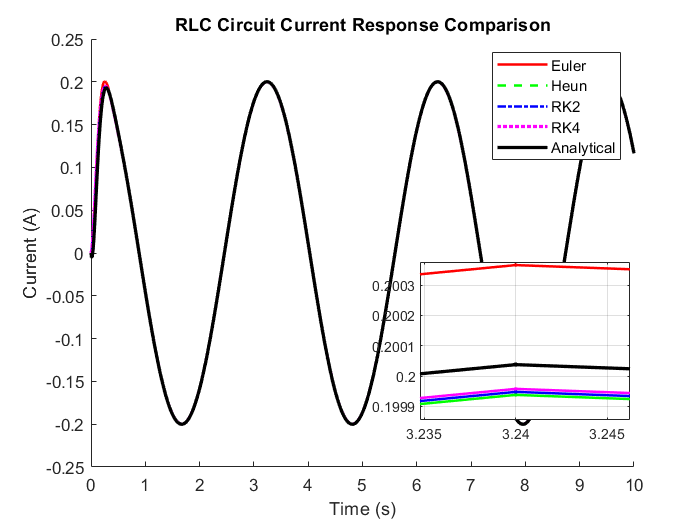
\includegraphics[width=0.81\linewidth]{Images/lab11}
		\caption{Current response in RLC circuit simulated using four numerical methods. The RK4 method (magenta) shows the smoothest response, while Euler's method (red) exhibits significant numerical oscillation.}
		\label{fig:results}
	\end{figure}
	
	\subsection{Discussion}
	The experiment successfully modeled a series RLC circuit and solved its governing differential equation using four numerical methods. Key observations:
	
	\begin{itemize}
	
		
		\item \textbf{Method Comparison}:
		\begin{enumerate}
			\item \textit{Euler's method} showed significant error accumulation and oscillation, especially during rapid changes in current
			\item \textit{Heun's method} provided moderate improvement but still exhibited phase errors
			\item \textit{RK2 method} demonstrated good balance between accuracy and computation
			\item \textit{RK4 method} produced the most accurate and stable solution
		\end{enumerate}
		
	
	\end{itemize}
	
 While Euler's method is simplest to implement, its accuracy limitations make it unsuitable for sensitive electrical system simulations. For most engineering applications, RK4 provides the best compromise between accuracy and computational requirements. This experiment demonstrates how numerical methods enable analysis of complex electrical systems that lack closed-form solutions.
\end{document}